\FloatBarrier
\subsubsection{Analysing IQ-data: Figures of merit}




\begin{figure}
\centering
{\includegraphics[width=12.9cm]{plots/IQ_plots/figures_of_merit/awesome_multiplot.pdf}}
\caption{
IQ-measurement with $T_{mes} = \SI{640}{ns}$ at $P_{mes} = \SI{24}{dBm}$ and $330000$ points. The scatter plot shows the first $10000$ data points with an alpha value of $0.1$. The circles represent the $2\sigma$-radius of the gaussian profiles obtained by fitting the 2D-histogram as described above. The histograms are computed by binning the $I$- respectively the $Q$-component of each individual measurement record of the full data set into $50$ intervals of equal length. The coloured lines again show the gaussian profiles of the corresponding disk, as achieved from fitting the 2D-model, but the amplitude is corrected by a scaling factor of $\sqrt{2 \pi \sigma^2}$ times the bin-width to account for the projection onto the respective axis.
}
\label{fig:IQ:figures_of_merit:awesome_multiplot}
\end{figure}









\begin{figure}
\centering
\subcaptionbox{
Scatter plot of the IQ-data with $2\sigma\text{-radius}$ of the fitted gaussian profiles.
\label{fig:IQ:figures_of_merit:scatter}}
[8.6cm]{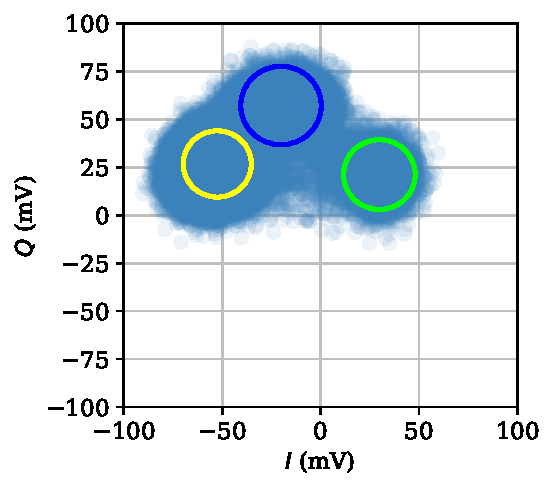
\includegraphics[width=8.6cm]{plots/IQ_plots/figures_of_merit/scatter_plot.pdf}}
~
\subcaptionbox{
Logarithmic histogram of the binned IQ-data.
\label{fig:IQ:figures_of_merit:2D_histo}}
[8.6cm]{\includegraphics[width=8.6cm]{plots/IQ_plots/figures_of_merit/histo_log.pdf}}
~
\subcaptionbox{
Cumulative projection of the binned data onto the $Q$- and $I$-axis and the gaussian envelopes of the respective disks. The colors are the same as in (\subref{fig:IQ:figures_of_merit:scatter}), the sum of the three gaussians is shown in red.
\label{fig:IQ:figures_of_merit:projected_histo_lin}}
[8.6cm]{\includegraphics[width=8.6cm]{plots/IQ_plots/figures_of_merit/projected_histo_lin_combined_plot.pdf}}
~
\subcaptionbox{
Projection of the logarithmic histogram. Does this even make sense?
\label{fig:IQ:figures_of_merit:projected_histo_log}}
[8.6cm]{\includegraphics[width=8.6cm]{plots/IQ_plots/figures_of_merit/projected_histo_log_combined_plot.pdf}}
\caption{
IQ-measurement with $T_{mes} = \SI{640}{ns}$ at $P_{mes} = \SI{24}{dBm}$ and $330000$ points. In order to quantify the separation and the spread of the disks, that represent the different quantum states, I bin the results onto a 2D-histogram and perform a least-square-fit with the sum of three gaussian profiles.
}
\label{fig:IQ:figures_of_merit:main}
\end{figure}







\FloatBarrier
\subsubsection{Readout Power Sweep}

%
%
%\begin{figure}
%\centering
%\subcaptionbox{
%caption 111
%\label{fig:IQ:improving_contrast:readout_power:1}}
%[4.0cm]{\includegraphics[width=4.0cm]{plots/IQ_plots/contrast_sweeps/readout_power/3dBm.pdf}}
%~
%\subcaptionbox{
%caption 111
%\label{fig:IQ:improving_contrast:readout_power:2}}
%[4.0cm]{\includegraphics[width=4.0cm]{plots/IQ_plots/contrast_sweeps/readout_power/6dBm.pdf}}
%~
%\subcaptionbox{
%caption 111
%\label{fig:IQ:improving_contrast:readout_power:2}}
%[4.0cm]{\includegraphics[width=4.0cm]{plots/IQ_plots/contrast_sweeps/readout_power/9dBm.pdf}}
%~
%\subcaptionbox{
%caption 111
%\label{fig:IQ:improving_contrast:readout_power:2}}
%[4.0cm]{\includegraphics[width=4.0cm]{plots/IQ_plots/contrast_sweeps/readout_power/12dBm.pdf}}
%~
%\subcaptionbox{
%caption 111
%\label{fig:IQ:improving_contrast:readout_power:2}}
%[4.0cm]{\includegraphics[width=4.0cm]{plots/IQ_plots/contrast_sweeps/readout_power/15dBm.pdf}}
%~
%\subcaptionbox{
%caption 111
%\label{fig:IQ:improving_contrast:readout_power:2}}
%[4.0cm]{\includegraphics[width=4.0cm]{plots/IQ_plots/contrast_sweeps/readout_power/18dBm.pdf}}
%~
%\subcaptionbox{
%caption 111
%\label{fig:IQ:improving_contrast:readout_power:2}}
%[4.0cm]{\includegraphics[width=4.0cm]{plots/IQ_plots/contrast_sweeps/readout_power/21dBm.pdf}}
%~
%\subcaptionbox{
%caption 111
%\label{fig:IQ:improving_contrast:readout_power:2}}
%[4.0cm]{\includegraphics[width=4.0cm]{plots/IQ_plots/contrast_sweeps/readout_power/24dBm.pdf}}
%\caption{main caption}
%\label{fig:jpc:noise_rise:main}
%\end{figure}
%

\FloatBarrier
\subsubsection{Readout Time}

%
%\begin{figure}
%\centering
%\subcaptionbox{
%caption 111
%\label{fig:IQ:improving_contrast:readout_time:1}}
%[4.0cm]{\includegraphics[width=4.0cm]{plots/IQ_plots/contrast_sweeps/readout_time/80ns.pdf}}
%~
%\subcaptionbox{
%caption 111
%\label{fig:IQ:improving_contrast:readout_time:1}}
%[4.0cm]{\includegraphics[width=4.0cm]{plots/IQ_plots/contrast_sweeps/readout_time/160ns.pdf}}
%~
%\subcaptionbox{
%caption 111
%\label{fig:IQ:improving_contrast:readout_time:1}}
%[4.0cm]{\includegraphics[width=4.0cm]{plots/IQ_plots/contrast_sweeps/readout_time/320ns.pdf}}
%~
%\subcaptionbox{
%caption 111
%\label{fig:IQ:improving_contrast:readout_time:1}}
%[4.0cm]{\includegraphics[width=4.0cm]{plots/IQ_plots/contrast_sweeps/readout_time/640ns.pdf}}
%\caption{main caption}
%\label{fig:jpc:noise_rise:main}
%\end{figure}
